\documentclass[a4paper]{article}
\usepackage[utf8]{inputenc}
\usepackage[spanish, es-tabla]{babel}

\usepackage{amsmath}
\usepackage{amsfonts}
\usepackage{amssymb}

\usepackage{float}
\usepackage{graphicx}
\graphicspath{ {./Imagenes/} }

\usepackage{multirow}
\setlength{\doublerulesep}{\arrayrulewidth}

\usepackage{array}
\newcolumntype{C}[1]{>{\centering\let\newline\\\arraybackslash\hspace{0pt}}m{#1}}

\usepackage[american]{circuitikz}

\usepackage{fancyhdr}

\usepackage{units} 

\pagestyle{fancy}
\fancyhf{}
\lhead{22.01 Teoría de Circuitos}
%\rhead{Mechoulam, Lambertucci, Rodriguez, Londero, Galdeman}
\rfoot{Página \thepage}



\begin{document}

%%%%%%%%%%%%%%%%%%%%%%%%%%%%%%%%%%%%%%%%%%%%%%%%%%%%%%%%%%%%%%%%%%%%%%%%% 
%								CARATULA								%
%%%%%%%%%%%%%%%%%%%%%%%%%%%%%%%%%%%%%%%%%%%%%%%%%%%%%%%%%%%%%%%%%%%%%%%%% 

\begin{titlepage}
\newcommand{\HRule}{\rule{\linewidth}{0.5mm}}
\center
\mbox{\textsc{\LARGE \bfseries {Instituto Tecnológico de Buenos Aires}}}\\[1.5cm]
\textsc{\Large 22.01 Teoría de Circuitos}\\[0.5cm]


\HRule \\[0.6cm]
{ \Huge \bfseries Trabajo práctico N$^{\circ}$5}\\[0.4cm] 
\HRule \\[1.5cm]


{\large

\emph{Grupo 3}\\
\vspace{3px}

\begin{tabular}{lr} 	
\textsc{Mechoulam}, Alan  &  58438\\
\textsc{Lambertucci}, Guido Enrique  & 58009 \\
\textsc{Rodriguez Turco}, Martín Sebastian  & 56629 \\
\textsc{Londero Bonaparte}, Tomás Guillermo  & 58150 \\
\textsc{Galdeman}, Agustín & 59827\\
\end{tabular}

\vspace{20px}

\emph{Profesores}\\
Jacoby, Daniel Andrés\\
Belaustegui Goitia, Carlos\\
Iribarren, Rodrigo Iñaki\\
\vspace{3px}
%\textsc{} \\	

\vspace{100px}

\begin{tabular}{ll}

Presentado: & */*/19\\

\end{tabular}

}

\vfill

\end{titlepage}


%%%%%%%%%%%%%%%%%%%%%%%%%%%%%%%%%%%%%%%%%%%%%%%%%%%%%%%%%%%%%%%%%%%%%%%%% 
%								INFORME									%
%%%%%%%%%%%%%%%%%%%%%%%%%%%%%%%%%%%%%%%%%%%%%%%%%%%%%%%%%%%%%%%%%%%%%%%%%

\section{Introducción}

En el presente informe se estudiaron distintos tipos de filtros con un enfoque analítico, teórico, práctico y además computacional. Para facilitar esto último se creó una interfaz gráfica que logra superponer distintas curvas obtenidas mediante cálculos teóricos de transferencias, mediciones con osciloscopio o simulaciones con LTSpice.

\section{Desarrollo}

\subsection{Ejercicio 1: Filtro Twin T Notch}
\subsubsection{Introddución}
Se diseñó el filtro Twin T Notch mostrado en la Figura (\ref{fig:filtroinicial}). El cual es implementado a traves de 2 filtros puestos en paralelo siendo uno pasa-Bajos y el otro pasa-Altos .

\begin{figure}[H]
	\centering
	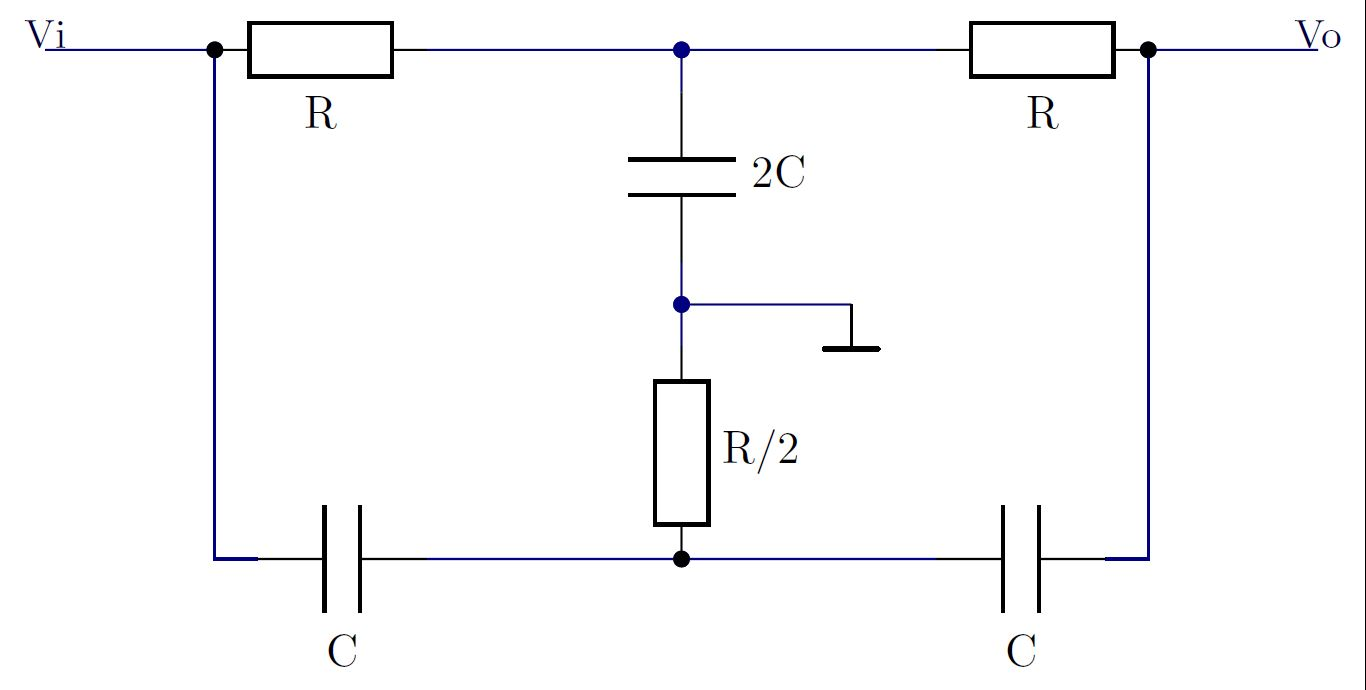
\includegraphics[width=0.7\textwidth ,trim={0 0.1cm  0.5cm 0},clip]{ej1inicial.jpg}
\caption{Filtro Twin T Notch teórico, sin simplificar.}
	\label{fig:filtroinicial}
\end{figure}

\subsubsection{Cálculo Analítico}
En el circuito se puede observar dos circuitos T conectados en paralelo. Aplicando el teorema de Kennelly para transformar T a Pi, se obtiene el circuito simplificado de la Figura (\ref{fig:filtrosimplificado}), donde se tiene que
\[Z_1=\frac{1+SCR}{SC}\hspace{1em};\hspace{1em} Z_2=2R(1+SCR) \hspace{1em};\hspace{1em} Z'_2=\frac{2(SCR+1)}{R(SC)^2}\]

\begin{figure}[H]
	\centering
	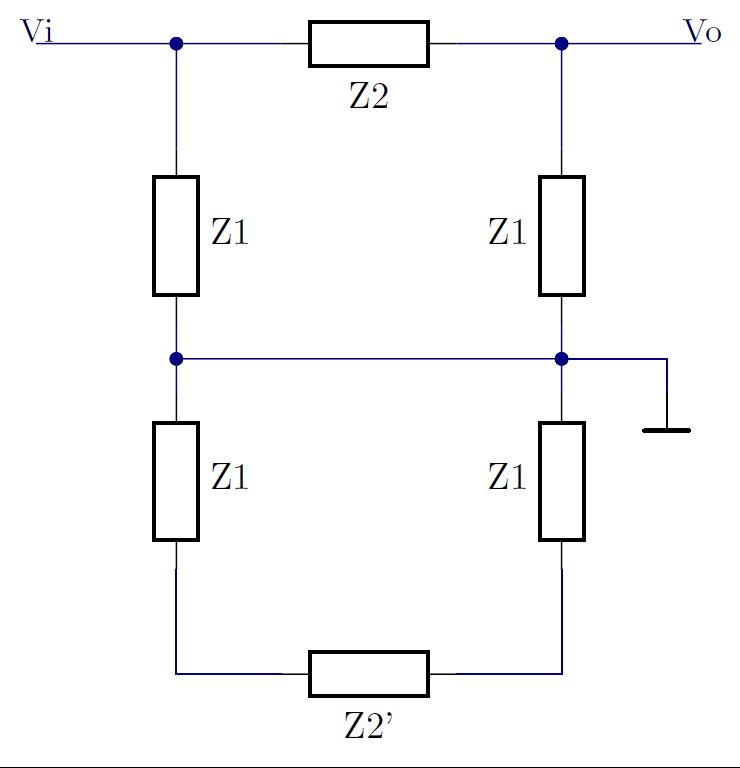
\includegraphics[width=0.6\textwidth, trim={0 0.1cm  0 0},clip]{ej1kennellly.jpg}
\caption{Filtro Twin T Notch luego de aplicar el teorema de Kenelly.}
	\label{fig:filtrosimplificado}
\end{figure}

Luego, se observa que el circuito puede simplificarse aún mas teniendo en cuenta que las dos impedancias $Z_1$ de la izquierda están en paralelo entre sí, de la misma forma que las $Z_1$ de la derecha y que $Z_2$ con $Z_2'$. Finalmente, se obtiene el circuito mostrado en la Figura (\ref{fig:filtrofinal}).

\begin{figure}[H]
	\centering
	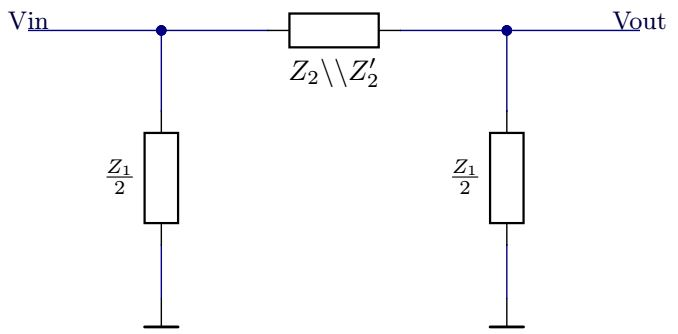
\includegraphics[width=0.6\textwidth]{ej1simplificado.jpg}
\caption{Filtro Twin T Notch simplificado.}
	\label{fig:filtrofinal}
\end{figure}

Realizando los cálculos de la transferencia en el circuito simplificado, se obtiene que
\begin{equation}
 \frac{Vo}{Vi}=H(S)=\frac{ \left( SCR \right)^2 + 1}{\left( SCR \right)^2 + 4SCR + 1}
 \label{equ:Hhdes}
\end{equation} 
Luego, la respuesta en frecuencia será
\begin{equation}
 H(j\omega)=\frac{ \left( j 2\pi f CR \right)^2 + 1}{\left( j 2\pi f CR \right)^2 + j 8\pi fCR + 1}
 \label{equ:Hdejomega}
\end{equation}
Antitransformando por Fourier, se obtiene la respuesta impulsiva
\begin{equation}
 h(t)=\delta \left( t \right) \ + \ \frac{2}{RC\sqrt{3}} \left[ \left( 2 + \sqrt{3} \right) e^{-t\frac{2 + \sqrt{3}}{RC}} + \left( \sqrt{3} - 2 \right) e^{t\frac{\sqrt{3} - 2}{RC}} \right]
 \label{equ:hdet}
\end{equation}
\subsubsection{Elección de componentes.}
 Este filtro posee una frecuencia de corte de $ 8.1 \ kHz $. Para eso se requerían resistencias de $ 8.9 \ k\Omega $ y $ 4.5 \ k\Omega $ y capacitores de $ 2.2 \ nF $ y $ 4.4 \ nF $.
Dado a que los componentes vienen limitados por los valores comerciales,  se seleccionaron resistencias de $ 6.8 \ k\Omega $ y $ 2.2 \ k\Omega $ en serie para obtener  $ 9 \ k\Omega $ y  resistencias de $ 10 \ k\Omega $ y $ 8,2 \ k\Omega $ en paralelo para formar $ 4.5 \ k\Omega $, mientras que para los capacitores, se eligieron 2 de $ 2.2 \ nF $ en paralelo para lograr los $ 4.4 \ nF $ deseados. Esto desplaza ligeramente la frecuencia de corte teniendo esta un nuevo valor de $f_c \approx 8.03 KHz$. Por lo tanto, en las ecuaciones mencionadas anteriormente, se considera $ R = 9 \ k\Omega $ y $ C = 2.2 \ nF $.\\
Previo a la puesta en practica del circuito se realizó una simulación de montecarlo para corroborar que por la dispersion provocada por las resistencias no haya mucha variacion en la frecuencia de corte; Obteniendo los siguientes gráficos:
\begin{figure}[H]
	\centering
	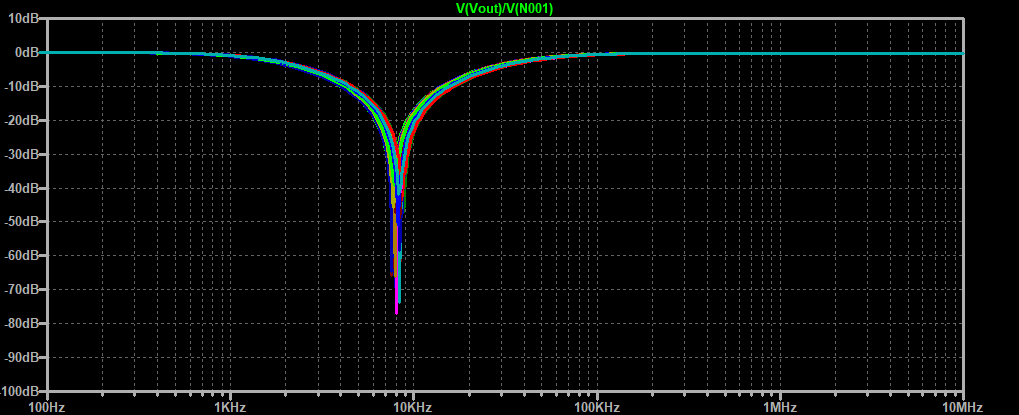
\includegraphics[width=\textwidth ]{Montecarlo.PNG}
\caption{Montecarlo Twin-T Notch Amplitud.}
	\label{fig:Montecarlo}
\end{figure}
\begin{figure}[H]
	\centering
	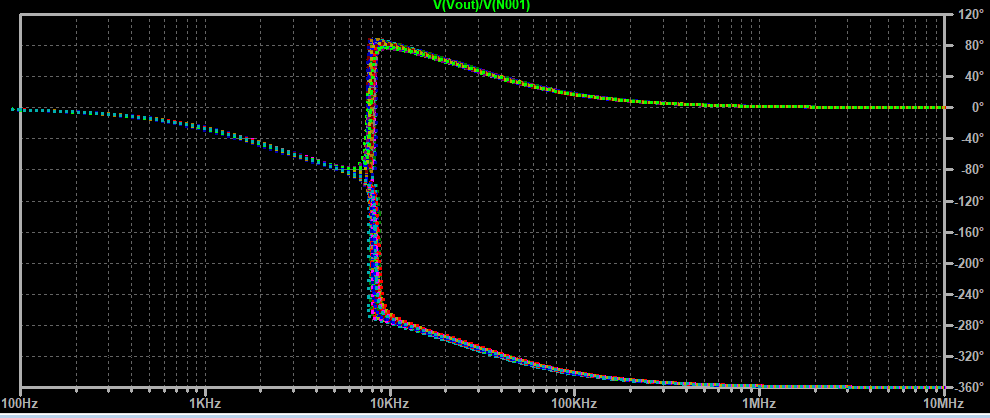
\includegraphics[width=\textwidth]{MontecarloPh.PNG}
\caption{Montecarlo Twin-T Notch Fase.}
	\label{fig:MontecarloFase}
\end{figure}
Se puede observar que la mayoria de las frecuencias de corte se encuentran en un entorno cercano a 8.1KHz
\subsubsection{Mediciones.}
Se midió el BODE de el circuito diseñado utilizando un generador de funciones y un osciloscopio, luego se hizo una simulación y se cotejó con el calculo teórico superponiendo los 3 gráficos:
\begin{figure}[H]
	\centering
	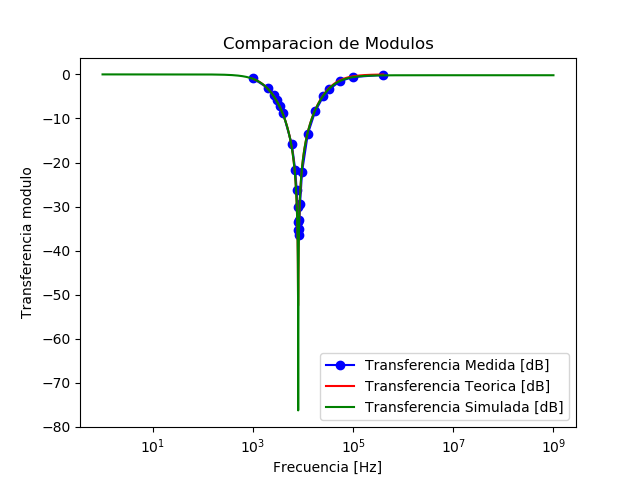
\includegraphics[width=0.6\textwidth, trim={0 0.1cm  0 0},clip]{BodeNotchAmp.png}
\caption{Bode Notch, Amplitud.}
	\label{fig:BodeNotchAmp}
\end{figure}
\begin{figure}[H]
	\centering
	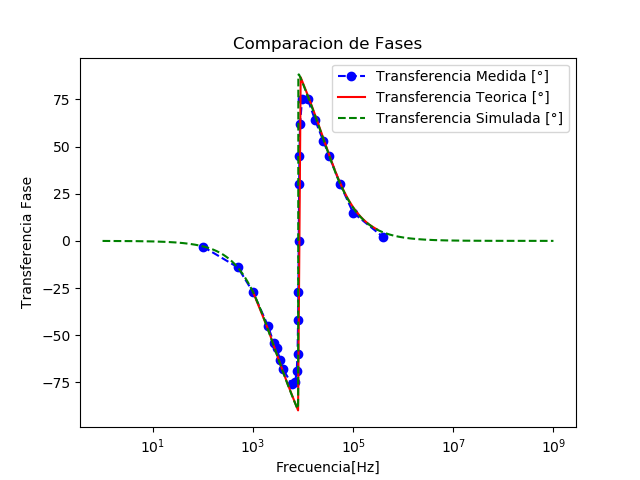
\includegraphics[width=0.6\textwidth, trim={0 0.1cm  0 0},clip]{BodeNotchPhase.png}
\caption{Bode Nothc, Fase.}
	\label{fig:BodeNotchPhase}
\end{figure}
Se puede apreciar que la frecuencia de corte es de aproximadamente 8.1KHz y que las mediciones coinciden con las simulaciones y las predicciones teoricas.
\subsubsection{Respuesta al escalon.}
Convolucionando con el escalón, se llega a la respuesta al escalón
\begin{equation}
 y(t) = \frac{2}{\sqrt{3}} \left( e^{-t\frac{2 + \sqrt{3}}{RC}} - e^{t\frac{\sqrt{3} - 2}{RC}} \right) + 1
\label{equ:h*u}
\end{equation} 
Luego se simuló y midio la respuesta al escalon con el siguiente grafico siendo la superposicion de los 3
\begin{figure}[H]
	\centering
	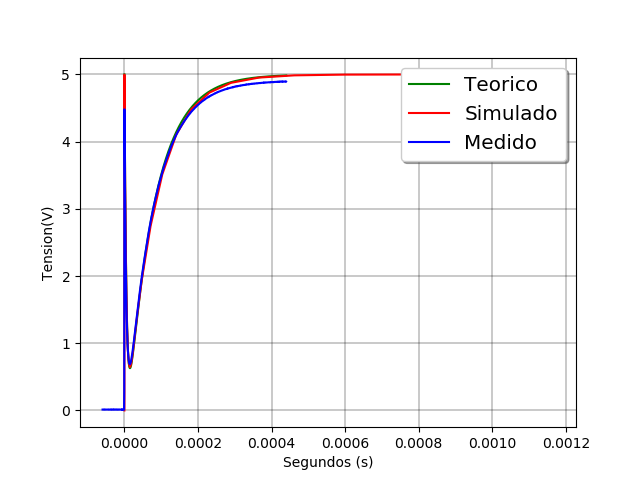
\includegraphics[width=0.9\textwidth]{StepResponse.png}
\caption{Respuesta al escalon.}
	\label{fig:stepResponse}
\end{figure}
Si bien lo simulado teórico y medido parecen coincidir en la mayoría, hay una zona donde no es así, y eso ocurre en la sección inicial, dado que en el modelo teórico la cuadrada es ideal y está compuesta por infinitas frecuencias, por lo que no hay problema con que llegue a la tensión máxima en el origen, mientras que en el caso real no es así. El generador de funciones no proporciona infinitas frecuencias, ademas de que le lleva cierto tiempo en realizar la transición de $0 \ V$ a $5 \ V$. Es por ello que no se llega a $5 \ V$ en el momento inicial.

\subsection{Ejercicio 2: Filtro pasa-bajos RC}
Se simuló y se armó en un protoboard un filtro pasa-bajos RC, seleccionando los valores de los componentes adecuados para lograr que la frecuencia de corte sea de $ 48 \ kHz $. Los componentes utilizados fueron dos resistencias, una de $22 \ \Omega$ y otra de $680 \ \Omega$, colocadas en serie, y un capacitor de $4.7 \ nF$, contemplando los valores comerciales.
Dicho circuito fue alimentado con una señal cuadrada de $ 10 \ V_{PP} $ con una frecuencia de $ 24 \ kHz $.
Simulando dicho circuito, se llegan a los resultados mostrados en la Figura (\ref{fig:simu2}).

\begin{figure}[H]
	\centering
	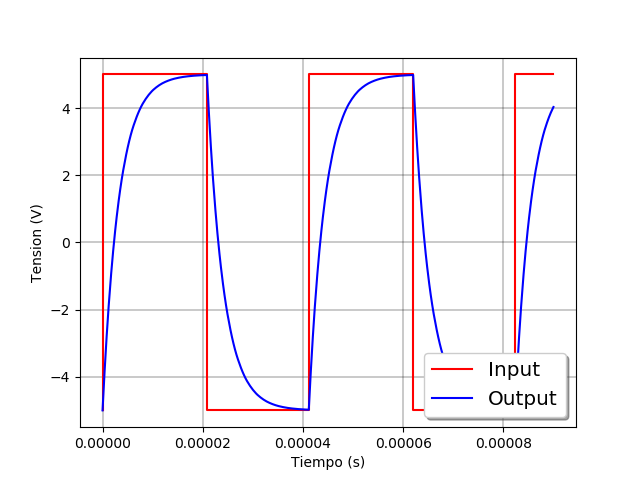
\includegraphics[width=0.9\textwidth]{Entrada-Salida.png}
\caption{Entrada (en azul) y salida (en amarillo) del circuito armado.}
	\label{fig:simu2}
\end{figure}

En este se observa que la salida no es igual a la entrada. Se encuentran dos formas posibles de explicar dicha observación. El primer enfoque viene dado de la mano de la carga del capacitor, la cual se sabe que no es instantánea , demorando así la obtención del valor pico. El segundo se basa en observar como afecta a los coeficientes de fourier de la entrada el circuito. Como se ha dicho previamente, este circuito es un pasa-bajos, por lo tanto, las frecuencias altas son atenuadas. Una señal cuadrada, idealmente, está compuesta por la suma de infinitas frecuencias, en la practica no son infinitas pero sí se puede asegurar que la conforma una gran suma de armónicos. De esta forma, al pasar por el filtro pasa bajos las altas frecuencias se ven atenuadas, lo cual  causa que la onda de salida no sea un cuadrada. La atenuación de los armónicos se muestra en la Figura (\ref{fig:armonicoscomparacion}), donde se son comparados con los de la entrada.

\begin{figure}[H]
	\centering
	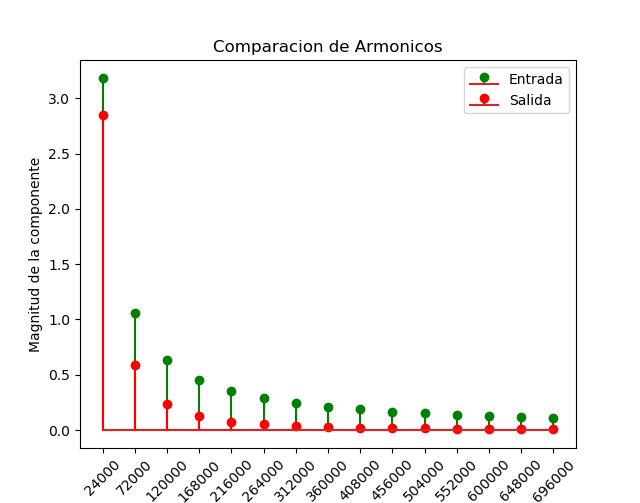
\includegraphics[width=0.9\textwidth]{ComparacionDeArmionicos}
\caption{Comparación de armónicos de la entrada (en verde) y salida (en rojo) del circuito armado.}
	\label{fig:armonicoscomparacion}
\end{figure}

Por otro lado, las mediciones se observan en la Figura (\ref{fig:medicion2}). Cabe destacar que en dicha figura, la señal cuadrada de la fuente no posee una forma cuadra perfecta debido a la baja impedancia de entrada de la fuente. Esta impedancia viene dada por el equivalente en serie de la resitencia y el capacitor
\[
	Z_{in} = R \ + \ \frac{1}{SC}
\]
donde se observa que es inversamente proporcional a la frecuencia. A altas frecuencias, el modulo de $Z_{in}$ disminuye y se hace mucho mas comparable con el de la fuente. A bajas frecuencias, como se observará en la Figura (\ref{fig:medicion2bajasf}), la impedancia de entrada aumenta, reduciendo la distorsión observada.

\begin{figure}[H]
	\centering
	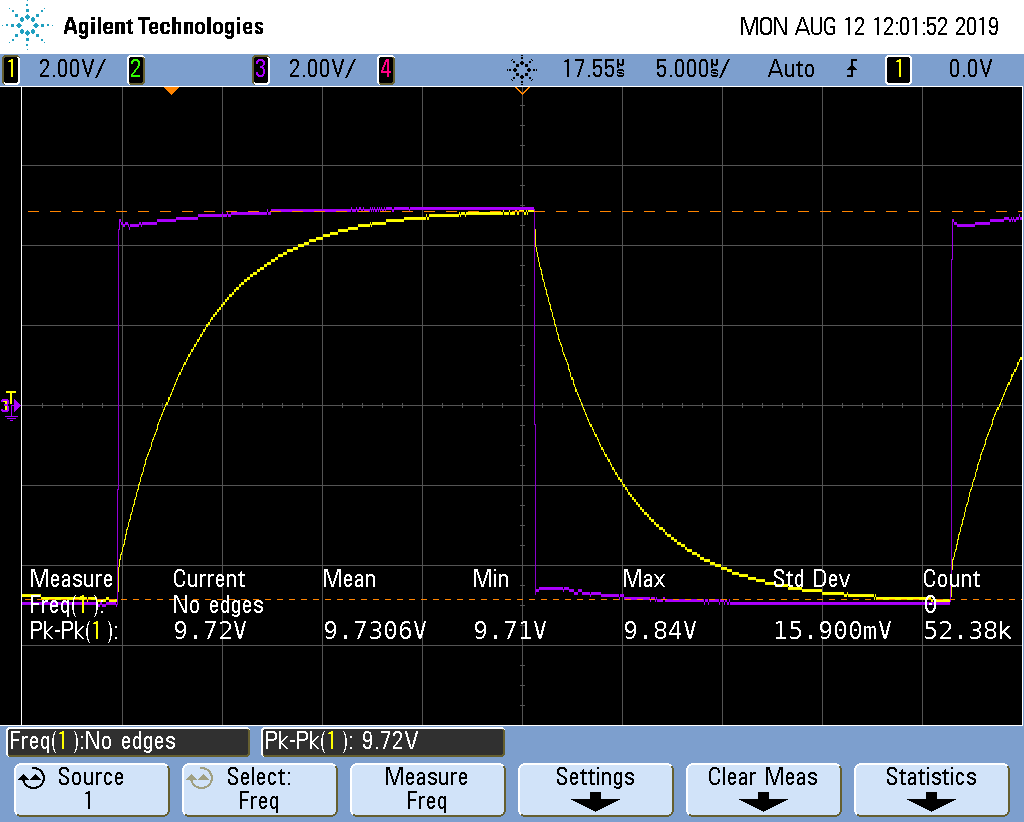
\includegraphics[width=0.9\textwidth , trim={0.7cm 6.25cm  0 3.5cm},clip]{scope_1}
	%trim={<left> <lower> <right> <upper>}
\caption{Entrada (en violeta) y salida (en amarillo) del circuito a $ 24 \ kHz $.}
	\label{fig:medicion2}
\end{figure}

De esta forma se puede comparar el diagrama de BODE teórico con el real observando las Figuras (\ref{fig:bodecomparacion}) y (\ref{fig:fasecomparacion}).

\begin{figure}[H]
	\centering
	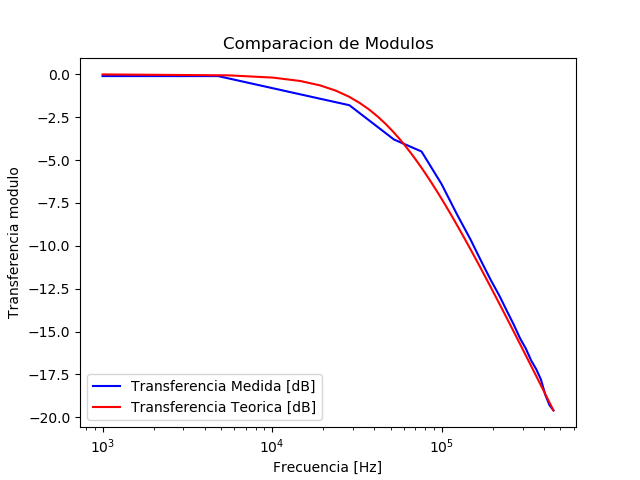
\includegraphics[width=0.8\textwidth]{BodeRealVsMedido}
\caption{Comparación del BODE real (en azul) con el teórico (en rojo).}
	\label{fig:bodecomparacion}
\end{figure}

\begin{figure}[H]
	\centering
	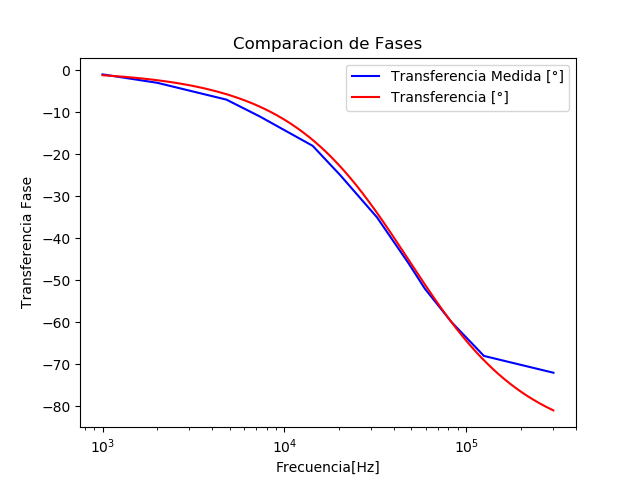
\includegraphics[width=0.8\textwidth]{FaseRealVsMedido}
\caption{Comparación de las fases del BODE real (en azul) con el teórico (en rojo).}
	\label{fig:fasecomparacion}
\end{figure}

En ambas figuras es posible ver que las mediciones se corresponden a los valores esperados, dejando pasar las frecuencias bajas y atenuando las altas. La distorsión entre las fases que se observa en la parte inferior de la Figura (\ref{fig:fasecomparacion}) se atribuye a las altas frecuencias. 

Graficando tanto el modulo de la respuesta en frecuencia en decibles y los armónicos calculados se obtiene la siguiente figura. Se puede apreciar en un  mismo grafico como son los armonicos a la entrada, y el nivel de atenuación causada por la transferencia sobre los armonicos de la salida.  

\begin{figure}[H]
	\centering
	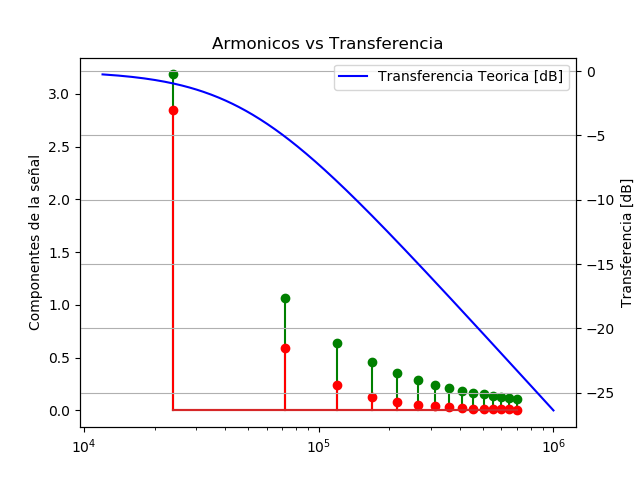
\includegraphics[width=0.8\textwidth]{ArmonicosVsTransferencia}
\caption{Grafico de transferencia y armónicos simulados.}
	\label{fig:aromincosvstransf}
\end{figure}

Repitiendo las mediciones con una señal de las mismas características, pero con una frecuencia de $ 480 \ Hz $ se observó que, a diferencia de lo observado en la Figura (\ref{fig:medicion2}), la señal de salida se acopla mejor a la entrada debido a que esta, al ser de baja frecuencia, no es atenuada como en el caso anterior.

\begin{figure}[H]
	\centering
	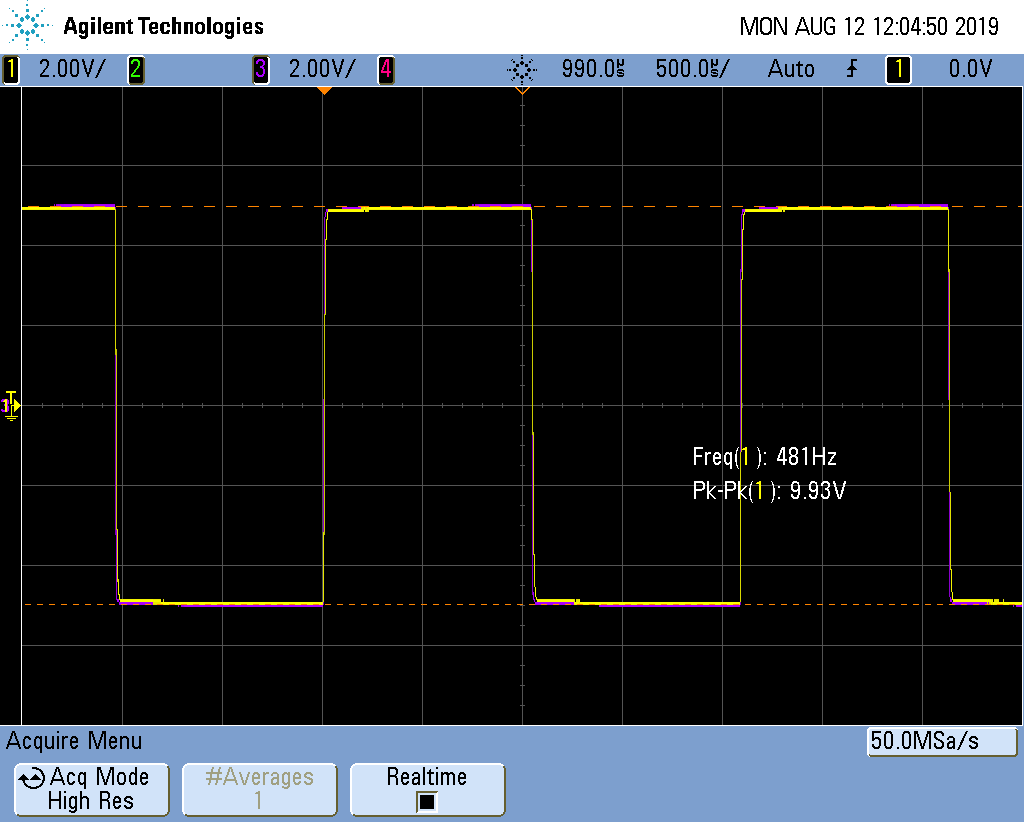
\includegraphics[width=0.9\textwidth , trim={0.7cm 6.25cm  0 3.5cm},clip]{scope_3}
	%trim={<left> <lower> <right> <upper>}
\caption{Entrada (en violeta) y salida (en amarillo) del circuito a $ 480 \ Hz $.}
	\label{fig:medicion2bajasf}
\end{figure}

Finalmente, se puede observar que dicho circuito puede ser utilizado como un integrador atenuado a muy altas frecuencias, ya qué

\begin{equation}
	H \left(S \right) = \frac{1}{SRC \ + 1} \approx \frac{1}{RC} \cdot \frac{1}{S}
\end{equation}
El sistema quedara defindo por 
\begin{equation}
	Y \left(S \right) = X \left(S \right) \cdot \frac{1}{S} \cdot \frac{1}{RC}
\end{equation}
Al antitransformar la expresión queda 
\begin{equation}
	y \left(t \right)=\int_{0}^{t} \frac{1}{RC}\cdot x(\tau) d\tau
\end{equation}
Esto se llevó a la practica y se midio la entrada versus la salida a una frecuencia  de  200KHz , asi concluyendo que realmente actua como integrador.
\begin{figure}[H]
	\centering
	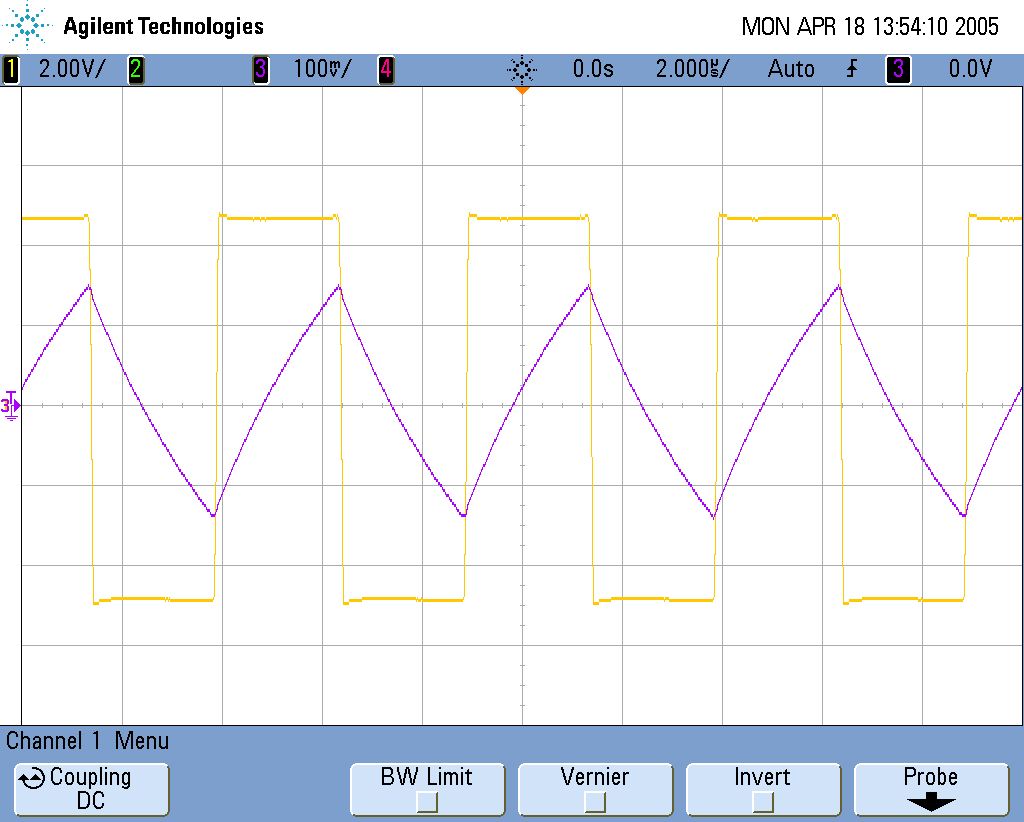
\includegraphics[width=0.8\textwidth,trim={0.7cm 6.25cm  0 3.5cm},clip]{Integrando.png}
\caption{Filtro pasa bajos actuando como Integrador.}
	\label{fig:integrand}
\end{figure}
\subsection{Ejercicio 3: Plot Tool 2019}
Finalmente, en este punto se programó una GUI en Phyton que permite realizar gráficos de diagramas de BODE. Dicho programa permite analizar funciones transferencia analíticas, archivos de LTSpice, entre otros tipos de archivos. Esta interfaz facilita el estudio, análisis y comparación de los distintos diagramas.

\end{document}
